\documentclass[twocolumn,linenumbers]{aastex631}
%%\documentclass[linenumbers]{aastex631}
%%\documentclass[modern]{aastex631}
%%\documentclass[twocolumn]{aastex631}
\newcommand{\vdag}{(v)^\dagger}
\newcommand\aastex{AAS\TeX}
\newcommand\latex{La\TeX}

\usepackage{mathtools, graphicx, booktabs, apjfonts, soul, multirow}
%\addbibresource{Bibliography.bib} %For bibliography

\begin{document}

\title{The Cohesive Object Sequence: Continuity in the Mass-Density Distribution From Asteroids to Stars
\footnote{April, 21, 2025}}

\author[0000-0002-8482-4669]{Gabriel M Steward}
\affiliation{University of Idaho, Moscow, Idaho 83844}

\author[0000-0002-8592-0812]{Matthew Hedman}
\affiliation{University of Idaho, Moscow, Idaho 83844}

\begin{abstract}

There are many different kinds of astrophysical objects, ranging from asteroids to icy moons to gas giants to supergiant stars. However, most of these objects are usually studied in isolation. In this paper, we collect data for mass, radius, density, and surface gravity for over two thousand so-called ``cohesive objects.'' That is, objects with components in direct physical contact. We show that the majority of these objects fall on a ``cohesive object sequence'' with continuous links from one kind of an object to another, all the way from asteroids to the largest stars. From this sequence we identify where there are clear differences between object classifications, where such distinctions are lacking, as well as unusual trends among the objects that connect various kinds together. We also note which objects are not on this cohesive object sequence--primarily compact stellar remnants. The primary result of this research is a single large plot intended to be spread around the astronomy and astrophysics community to showcase the connectedness of the universe and to identify object regimes that would benefit from collaboration among subfields.

\end{abstract}

\keywords{KEYWORDS (111) --- KEYWORDS (112)}

\section{Introduction} \label{sec:intro}

\textbf{\color{red} [NOTE: For major notes.] \color{black}}

\textbf{\color{red} [NOTE: Not sure what to put for Keywords...?] \color{black}}

The HR (Hertzsprung-Russel) diagram is a familiar sight to many. The relation of color temperature to luminosity succinctly shows how a simple relation of two observed quantities can be used to identify, categorize, and explain objects in space. The success of the HR diagram is difficult to overstate, as it is a cornerstone of astronomy and astrophysics courses. 

In recent years, a similar endeavor has been undertaken for exoplanets. Now that we have over 5000 confirmed discoveries, mass-radius plots can be constructed that show distinct domains of planetary types \citep{Chen2016, Muller2024}. These graphs, while similar in purpose and scope to the HR diagram, are not yet as successful, but likely will be in the future. One can also find similar distribution graphs for asteroids, such as mass-density plots \citep{Carry2012}. 

One may be tempted to think that these three domains of stars, exoplanets, and asteroids are entirely unrelated. However, that is not the case; all of them share some simple, basic properties. They are cohesive objects; that is, objects made of components in physical contact with each other, as opposed to non-cohesive objects like nebulae or galaxies. Each cohesive object has a particular mass and size, from which density and surface gravity can be determined. This means that every one of these objects can be placed on the same plot so long as two of the aforementioned values are used. 

In this paper, we present such a graph that plots the mass-density relation for all cohesive objects that we have decent measurements for, ranging from minuscule asteroids to supermassive black holes. The intention is that this plot will be shared readily among the community as a way to examine the overall distribution of objects in the universe, connecting many disciplines across astrophysics. Like the HR diagram, this distribution plot suggests many clear divisions by which to categorize objects, and even has a "main sequence" of sorts on which the vast majority of objects fall: the ``cohesive object sequence.'' 

We begin with \textbf{Results} since the primary result of this paper is the driving force behind it. \textbf{Discussion} of the distributions come next, including classification implications, outlier examinations, and connections between seemingly distinct objects. The \textbf{Conclusion} of our work follows, though afterward we describe the \textbf{Methods} used to gather and pair down the data. 

\section{Results} \label{sec:intro}

\begin{figure*}[htbp]
\centering
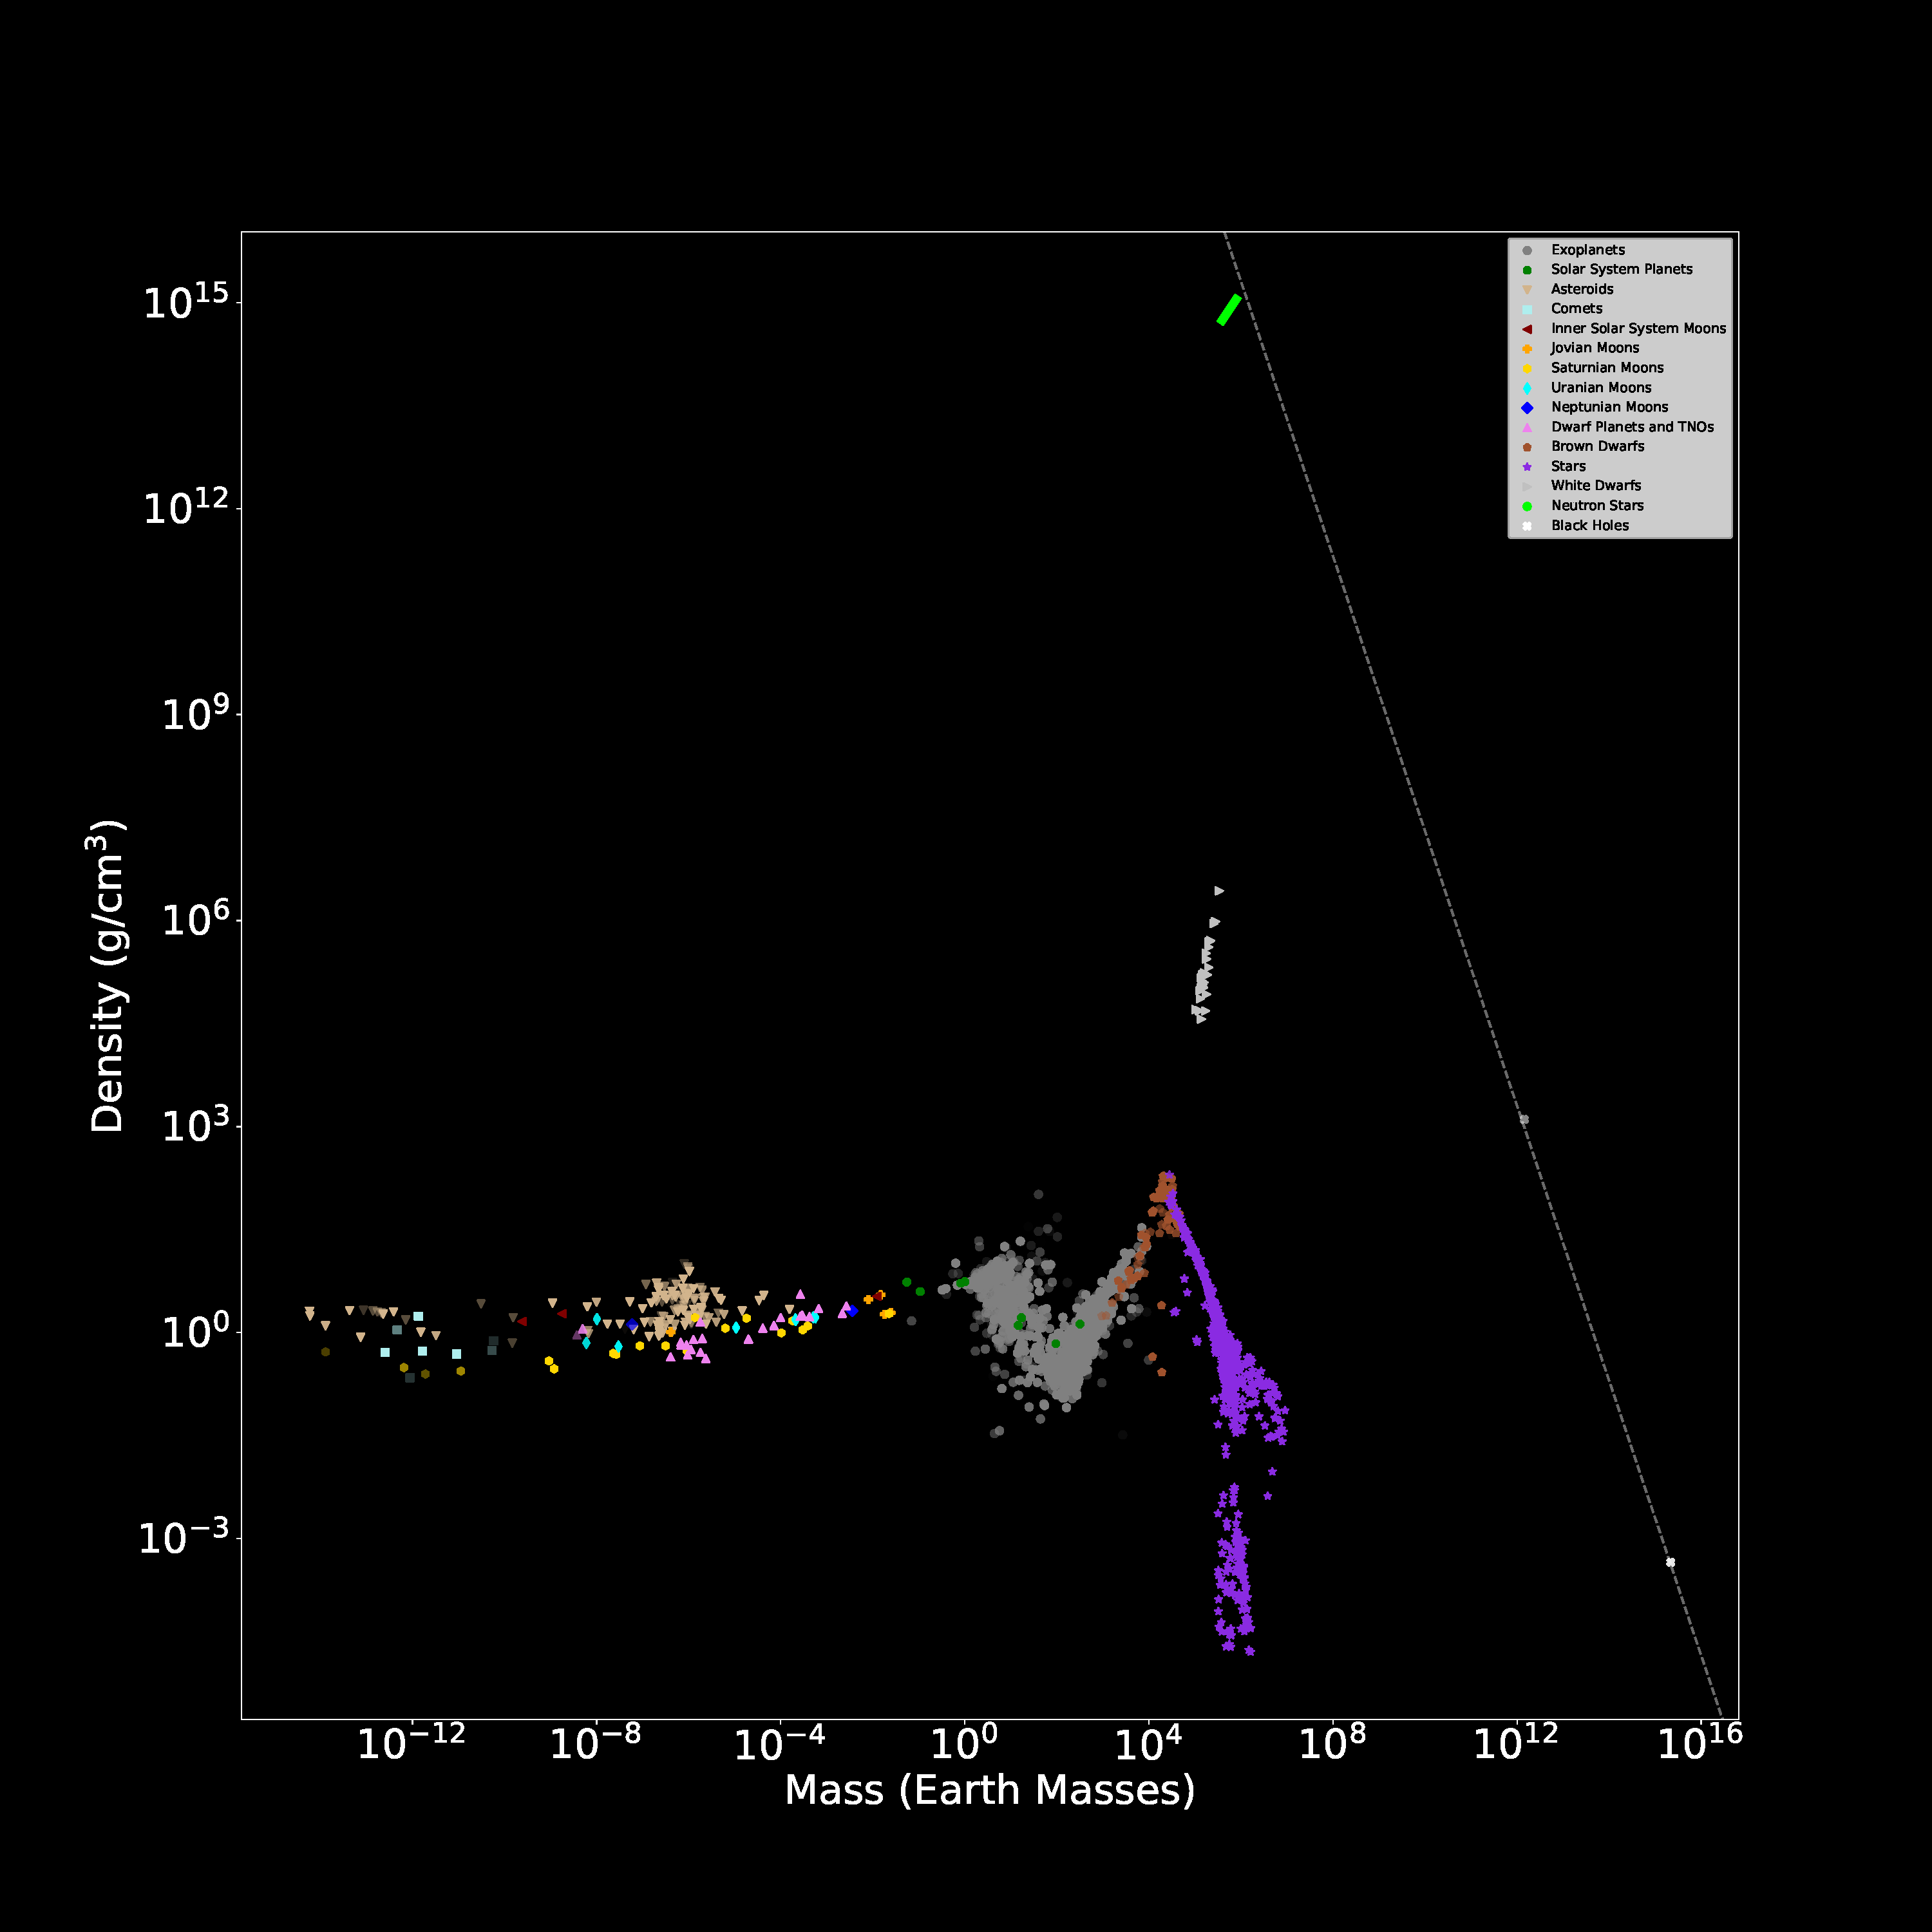
\includegraphics[scale = 0.35]{MassDensityPlot.pdf}
\centering
\caption{The relationship between density (in g/cm$^3$) and mass (in Earth masses) for cohesive objects in the universe on a log-log scale. Each kind of object is given a unique color and shape. The transparency of each point represents how large the errors are: solid objects have minimal errors while the more transparent ones have larger errors with a maximum relative permitted error of 0.5 in either mass or volume, whichever was larger for the object in question. As no neutron star radii have been measured to sufficient precision, the general area Neutron Stars occupy is given by a green line. The dashed line represents the Schwarzchild black hole event horizon limit, any object that reaches this line should theoretically collapse into a black hole.}
\label{fig:1}
\end{figure*}

Figure \ref{fig:1} is our primary result, showing the relation of mass and density for asteroids, comets, trans-Neptunian objects, moons, planets, brown dwarfs, stars, neutron stars, and black holes. Every data point represents a real object in the scientific literature. The points are categorized by type via shape and color. Classification was assigned based on the source they were found in. Transparency represents the relative error associated with each object: low errors plot solid points, while high errors are almost transparent. The maximum relative error plotted is 0.5 measured against the mass or volume, whichever was larger. Direct radius relative error was not used as mass correlates with radius cubed, and so the error propagation differs between the two by a factor of 3. The largest permitted errors are particularly noteworthy on outlier exoplanets, outlier asteroids, and relatively small objects. 

No neutron stars have had their radii measured with sufficient precision as far as we are aware. Thus, a loose range of neutron star masses and densities are plotted as a fat line, rather than individual points. Two black hole event horizon radii have been satisfactorily measured. To put them in context we opted to plot the theoretical mass-density relation for Schwarzchild black holes. The real-world observations line up remarkably well with the theoretical predictions here.

One may argue that a black hole is not really a ``cohesive object'' in the way they are considered here, as the event horizon is not a boundary of physical matter. (Most likely, there are debates on this point, see \cite{Mann2022}). However, black holes are certainly singular objects that appear as black orbs to an outside observer, so we choose to treat them as such. Strictly speaking, what is measured is an apparent horizon; it is impossible to measure the true event horizon in all but highly idealized cases \citep{Visser2014}. However, as we can see from Figure \ref{fig:1}, the measured values of the apparent horizons give results that line up closely with the theoretical event horizon's results, indicating that the distinction is unimportant in our case.

Expanded views of various sections of Figure \ref{fig:1} are shown in Figure \ref{fig:2}, examining four different mass scales. These views make it possible to pick out individual objects among the otherwise dense clouds.  

\begin{figure*}[htbp]
\centering
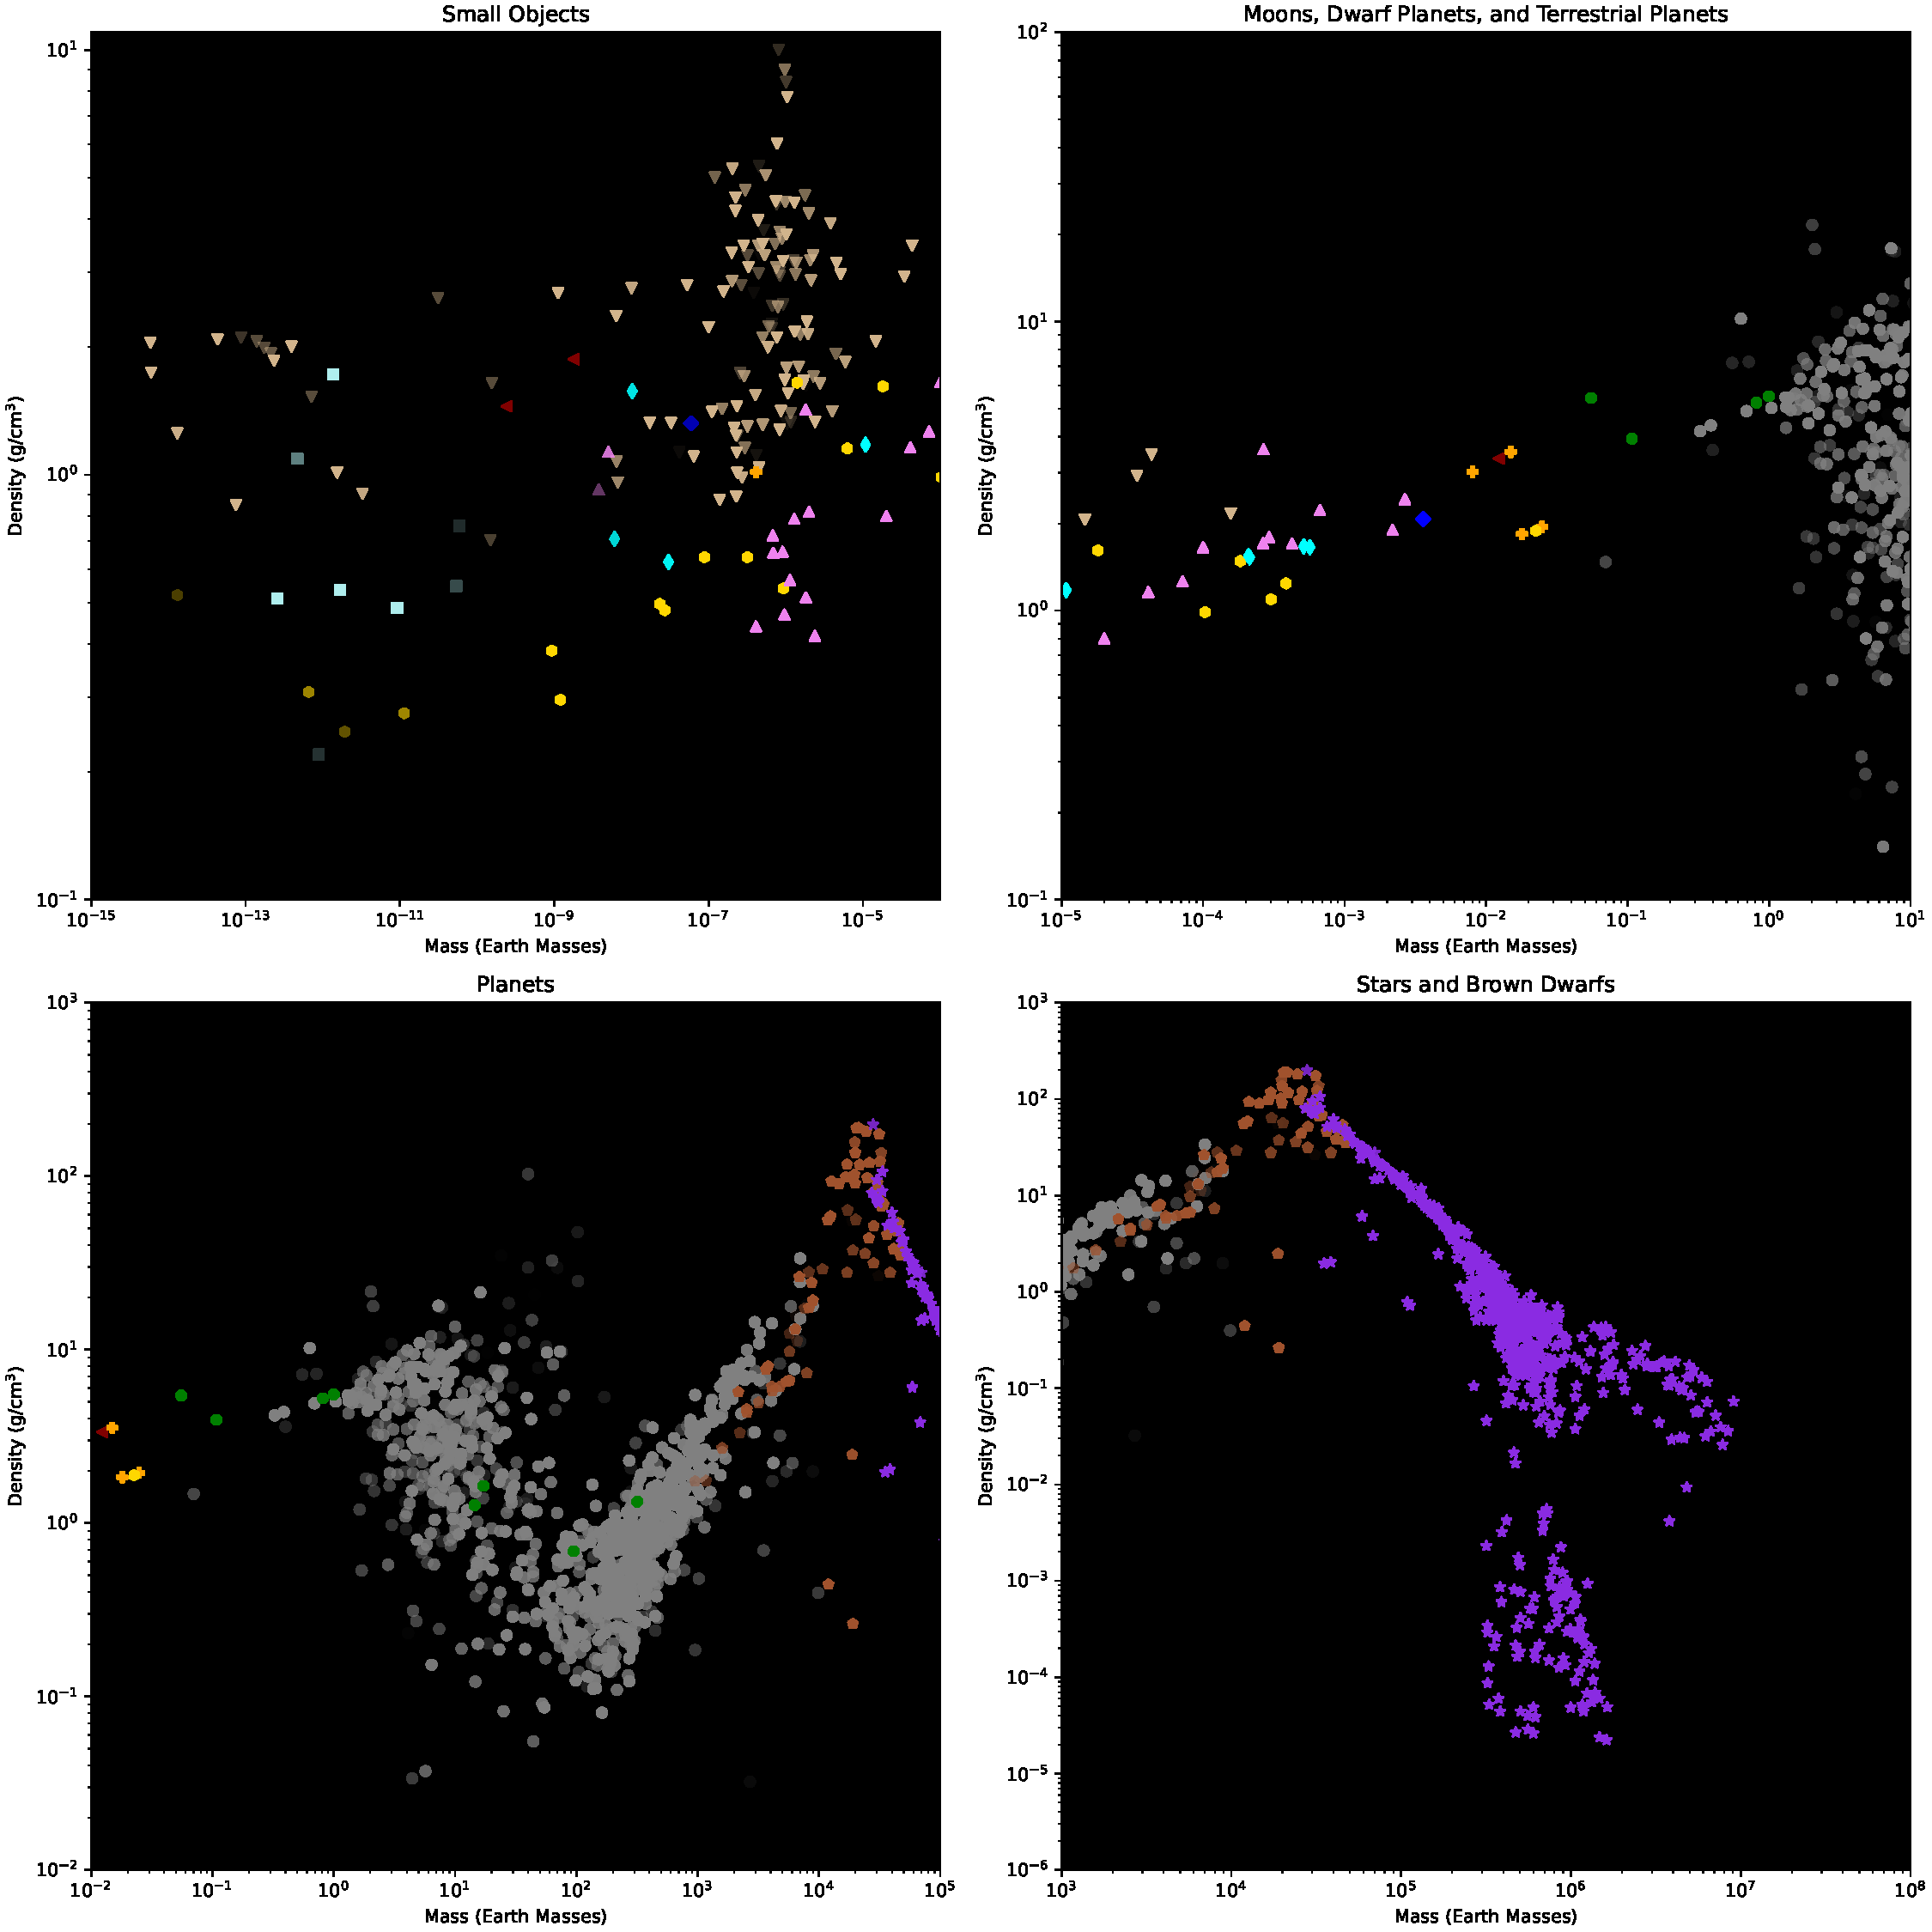
\includegraphics[scale = 0.45]{ZoomViews.pdf}
\centering
\caption{Zoomed in views of Figure \ref{fig:1} using the same colors and shapes. No view for white dwarfs or other extreme objects, as there is not much detail present in those ranges to begin with.}
\label{fig:2}
\end{figure*}

The actual data collected in our dataset are mass and radius, not mass and density. Mass and density were chosen for Figure \ref{fig:1} because it makes it easier to see distinct categories of objects, particularly in the lower-mass regime of exoplanets. However, the mass-radius relation is not ignored; we have it plotted in Figure \ref{fig:3} alongside other combinations of mass, radius, density, and surface gravity. 

\begin{figure*}[htbp]
\centering
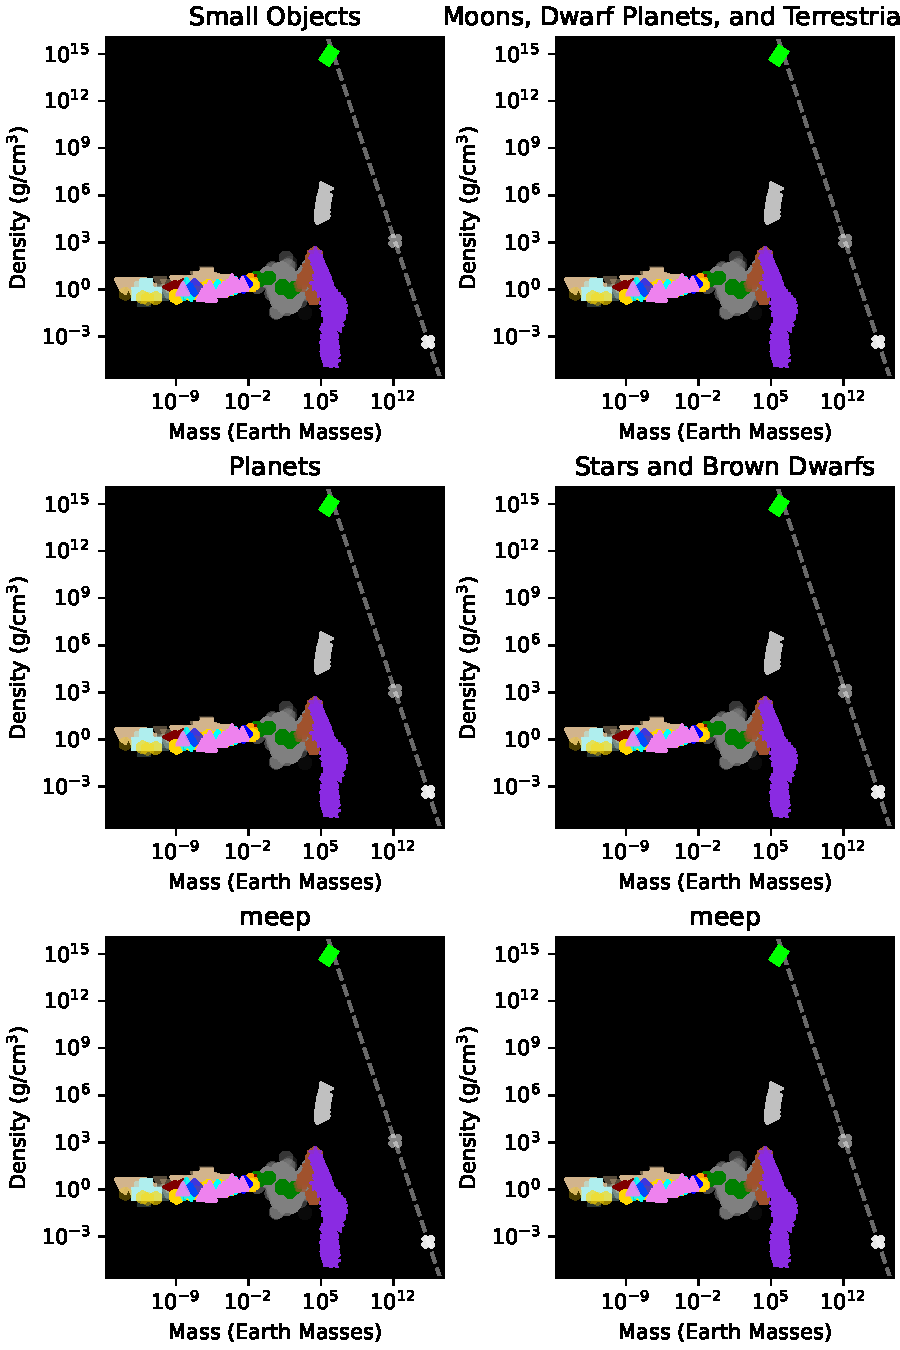
\includegraphics[scale = 1]{AltVariableViews.pdf}
\centering
\caption{Alternate views of the data set showing different combinations of mass, radius, density, and surface gravity. Colors and shapes are identical to Figure \ref{fig:1}.}
\label{fig:3}
\end{figure*}

\section{Discussion} \label{sec:intro}

Each area of Figure \ref{fig:1} reveals trends in the distribution of objects in the universe, and most of these smaller-scale trends have been noted by those studying those scales. As a whole, however, this graph showcases a seemingly unbroken progression from the smallest asteroids to the largest blue stars, cutting through most other kinds of objects along the way. We call this progression the ``cohesive object sequence'', after the stellar main sequence, which it contains. Of the objects considered here, only compact objects, giant stars, supergiant stars, and certain actively collapsing bodies lie off the cohesive object sequence.

One might be tempted to describe the cohesive object sequence as a description of how objects develop the more mass they accrete, but this should be avoided. Stars form from clouds of gas and have formed since before there were enough heavy elements to even make asteroids \citep{Maio2010}. One does not keep throwing asteroids at each other until fusion begins in nature. Another reason to avoid treating the cohesive object sequence as a description of development is that small objects can be created from larger ones. Many asteroids are fragments of once larger bodies \citep{Scott2020}, and terrestrial planets could have had extensive gaseous envelopes in the past that were blown off over time \citep{Kurokawa2014}. Formation pathways for objects of the same class can vary: larger gas giants could either form in a circumstellar disc or directly from a stellar nursery \citep{Schlaufman2018}. 

What the cohesive object sequence does show is that nature tends to form objects of certain masses out of certain materials. There are no rocky bodies the size of Jupiter. There are no gaseous objects the size of asteroids. And nothing less massive than a star is fusing any hydrogen (human activities excepted). 

Another key insight is that there tend to be smooth transitions between object classes at the extreme ends of those classes. Asteroids, trans-Neptunian objects, the Solar System's moons, and terrestrial planets all fall along a rather smooth gradient. Many objects sit right at the divide between terrestrial planets and volatile worlds (also known as ice giants). Even the sharp, well-defined transition between brown dwarfs and stars driven by the point of hydrogen fusion \citep{Boetticher2017} has smooth lines of data coming at it from both sides.

There are a handful of objects not on the cohesive object sequence. Naturally, there are the giant and supergiant stars that were deviations from the stellar main sequence in the first place; stars approaching the ends of their lives as they run out of hydrogen to burn. These have a transition zone where stars evolving to those final states lie. The supergiant stars contain the least dense objects in the universe--even less dense than the supermassive black hole M87*!

Speaking of black holes, the compact objects--white dwarfs, neutron stars, and black holes--are also not on the cohesive object sequence, and the jarring lack of objects connecting these regimes to the sequence is indicative of the dramatic processes that form them. (Though, notably, the difference between black holes and neutron stars is not very large). There is no "gradient" to becoming a compact object. That said, the distribution of white dwarfs does vaguely point away from the stars and toward neutron stars in a sort of tenuous link. 

The only other distinct class of object clearly off the cohesive object sequence are collapsing objects: very young stars, brown dwarfs, and gas giants that are inflated due to their recent formation \citep{Hartmann2016, Muller2021}. We do not have many of these objects plotted as we have measured so few of them, much like there are not many stars measured that are in the process of moving onto the supergiant stage of their lives. They simply do not spend enough time in these regimes for there to be a large population. Several of these young brown dwarves lie directly below the low end of the star mass regime, indicating that they may ignite once they compress further. 

Changing focus to examine the cohesive object sequence at smaller scales now, we can identify specific trends and how the object classes are related to each other. The first such visible trend is merely an illusion: there are very few tiny objects plotted, but a large number after about $10^{-8}$ Earth masses. This is not a real difference, there are far more tiny objects in the Solar System than there are larger ones; this is merely an observation bias since larger objects are easier to see. Many of the smallest objects plotted were visited by spacecraft, including the smallest, Itokawa \citep{Carry2012}. While we have lots of interplanetary dust samples that technically qualify as cohesive objects, they were deemed ``too small'' to bother including in the data set.

Dust accretes in protoplanetary discs to form planetesimals, though the exact process for doing so isn't well understood \citep{Blum2008}. Planetesimals, existing in the kilometer size regime, are found among the asteroids and trans-Neptunian objects in Figure \ref{fig:1}, though at the scale of the figure there is no way to differentiate what objects are true planetesimals and what were formed other ways, such as fragmentation. This is a somewhat common degeneracy among cohesive objects: formation pathway is not recoverable. 

The majority of plotted small objects cluster around $10^{-6}$ Earth masses, and here we can see a distinct difference between rocky objects and icy objects. The asteroids have generally larger densities than the trans-Neptunian objects and icy Saturnian moons. This is due largely to their material: ices are less dense than rock. The densest of asteroids are likely errors in measurement or reporting, as their density is slightly higher than that of pure iron. That said, there are no doubt some true metallic meteorites out there, due to fragmentation of a differentiated body \citep{Scott2020}. 

After an object obtains enough mass, it will begin to gravitationally round itself \citep{Stern2002, Lineweaver2010}. At the tail end of the cluster of asteroids, we reach the first object that is known to be gravitationally rounded in a normal manner, Saturn's icy moon Mimas. The largest irregular object, Vesta, is the second most massive asteroid, marking the point at which there are no more known irregular objects. These two objects only differ in mass by a single order of magnitude, but they nonetheless mark the change between irregular and spherical objects.

This change coincides with a peculiar trend: the range of densities between objects begins to narrow after gravitational rounding begins. There are no very dense asteroids of this size, but also no icy objects with particularly low densities. The trend manifests in a vaguely cone-like shape. This has been noticed before in the Kuiper belt \citep{Bierson2019} and can be seen in \cite{Carry2012} for asteroids, though in that case without the additional context from moons and trans-Neptunian objects the trend is not as obvious. \cite{Bierson2019} attribute the change over icy objects to gravitational compression and a subsequent loss of porosity, while we can logically deduce that for asteroids solid iron objects become less and less likely to form as size increases. The porosity argument no doubt applies to rubble-pile asteroids as well, it's just that these are denser than icy bodies to begin with.

With this, we reach the point in the data set with the least information, the realm of the largest dwarf planets, major moons of the Solar System, and the smallest planets. Pluto, Eris, and Triton cluster together, evidence of Triton's origin beyond Neptune \citep{Agnor2006}. Io, Europa, and the Moon all fall in a line, for they are largely rocky bodies, while Titan, Ganymede, and Callisto are in a separate, less dense line, being icy bodies. Mercury and Mars sit alone with few neighbors. After all, we are only now reaching the sensitivity required to detect these objects in other star systems, and most small exoplanet candidates did not pass through the error requirements we placed on our data. 

Extrapolation can still teach us about the smallest of planets, however. Mars lies in line with the larger Venus, Earth, and terrestrial exoplanets. Mercury does not, but it is well known that its density and metal content are unusually high \citep{Spohn2001}. It remains to be seen if such particularly dense small planets are regularly created in the universe, or if Mercury is truly an outlier. 

Debates as to what exactly a planet is have a long history \citep{Stern2002, Soter2006, Metzger2022} and sadly our research offers no help on the matter, as the objects near terrestrial planets fall along a rather clear line, with only minor differences between icy and rocky objects at the lower mass end. The transition from asteroids to Earthlike objects is smooth with no clear delineation. There is the general trend of lower density variation, but this is gradual. 

This is not the case once we exceed a few Earth masses. At this point, a far larger variety of densities open up to objects. We have now reached the boundary between terrestrial planets and volatile worlds. This is the least defined area of the cohesive object sequence; it is decidedly unclear where terrestrial planets end and volatile worlds begin. There is also some indication that there may be a handful of "water worlds" that exist in this region \citep{Adams2008, Zeng2019}, a type of planet that is neither terrestrial nor volatile--at least not in the same sense that Uranus and Neptune are volatile. The unfortunate reality is that planets in this uncertain range are extremely common and we do not have any examples of a planet in this regime within the Solar System. The true nature of this transition zone may remain mysterious for many more years. However, for all we cannot say about this region, we can say that it is continuous, and does not break off the cohesive object sequence in any significant manner--even the so-called ``radius valley'' \citep{Eylen2018, Armstrong2019}, which can be seen in Figure \ref{fig:2}'s zoom on the exoplanet region, is not a true divide as there are some objects that straddle it. 

It is worth noting that the volatile worlds themselves have the largest internal variation of any category on the entire cohesive object sequence. Almost everything else lies on narrow lines or at least regions with well-defined edges. Meanwhile, the volatile worlds have members of extremely high and low density across their entire mass range. There are even a handful of "overdense" worlds, some more massive than Uranus and Neptune, that have densities that may imply a potentially rocky composition, but there is currently no consensus as to what exactly these overdense worlds are \citep{Armstrong2020, Naponiello2023, Lange2024}. This highly variable density behavior drops off dramatically at the boundary between volatile worlds and gas giants, indicative of a distinct change in object character beyond just a distinction between the higher mass/lower density trend of volatile worlds and the higher mass/higher density trend of gas giants.

It just so happens that Saturn sits keenly in the middle of these two trends \citep{Ravit2023}, indicating that it is one of the smallest gas giants possible, or perhaps even a member of a thin transition zone. Below Saturn on the plot are a handful of volatile worlds and gas giants that are underdense--including planets inflated due to proximity to their stars \citep{Batygin2011}, and the so-called ``super-puffs'' \citep{Lee2016, Libby-Roberts2020}. In contrast, the cloud of overdense worlds is sharply cut off near the masses of the smallest gas giants, suggesting that it must be extremely difficult to form an object that massive and not accumulate a gaseous envelope. This makes sense when considering the gas giant formation mechanism; when planets forming in a gas-rich disc grow massive enough, they experience runaway gas accretion \citep{Bodenheimer1986, Venturini2016}. As gas is far more common in the universe than rocky/volatile material, it's difficult to imagine a situation with enough available rocky/volatile material and very little gas. 

Jupiter is a bog-standard example of a gas giant, right in the middle of lots of others found in the universe. As gas giants get more massive, they become denser with minimal change in physical size on a relatively predictable trajectory until they reach the masses required to start hydrogen fusion, and thus become stars \citep{Baraffe1998, Boetticher2017}. This leads us to the question of brown dwarfs: no matter which values are plotted, be they mass, radius, density, or surface gravity, there is no clear distinction between gas giants and brown dwarfs. The range of densities doesn't even change that much, as is the case when transitioning between asteroids and terrestrial planets. Brown dwarfs and gas giants are only colored differently in Figure \ref{fig:1} because of the sources they were drawn from, and there is a large overlap between the two classifications. From this, we see no reason to differentiate the two objects from each other, except possibly through formation pathway, but there is not a clear way to determine the method by which an object formed. The current default differentiator is the deuterium fusion burning limit \citep{Boss2007}, but we see no indication of that influencing the object on a demographic scale. 

Now that we've reached the definite end of all planets, it's time to take a look back. In every view of mass, radius, density, and surface gravity, there are three separate regimes for planets: terrestrial planets, volatile worlds, and gas giants. The clear distinctions between these three classes call into question the fact that they are traditionally considered the same kind of object when Earth has more in common with the asteroid Ceres than it does with Jupiter. This justifies the study of terrestrial planets, volatile worlds, and gas giants as their own distinct demographics, in addition to the collective approach we take throughout this paper. Popular science articles sometimes like to claim there is a fourth category, the ``super-Earth'' or ``sub-Neptune'', but the cohesive object sequence makes it clear that this population is either part of terrestrial planets, volatile worlds, or sits in a transition zone.

Stars follow the familiar pathways of the HR diagram, though they appear different when mass and density are considered. The trend of main sequence stars is higher mass, lower density. Low-mass stars have little variation in density, while high-mass stars show larger variability. Examination of the stars section in \ref{fig:3} shows a slight change in the mass-density slope between low-mass and high-mass stars, indicating that there may be some kind of fundamental difference between stars significantly more massive than the Sun and the demographic the Sun itself is in. The Sun itself is a completely normal member of the main sequence. The giant branch breaks off from the stellar main sequence at masses around that of the Sun and points toward the disconnected supergiant region. The stellar main sequence ends with blue stars, and the cohesive object sequence does not carry it into any further objects. Perhaps population III stars would extend the sequence further, but we have not conclusively observed them \citep{Larkin2022}.

Many objects are absent in the data. There are no doubt many smaller asteroids we have not properly measured. Plotting the tiny grains we have sampled would just needlessly extend the graph without any general benefit. Tiny planets and exomoons certainly exist, we just have not observed them. We also need to consider the fact that the Solar System may give us a biased sample of certain objects; it is possible our moons and dwarf planets are not typical, or that many systems simply won't have iron asteroids, or that the trend of larger icy objects being denser does not exist elsewhere. 

Despite these holes, the continuous connection between all the objects on the cohesive object sequence is clear. The universe is interconnected across almost all scales. This includes scales not presented on this graph: interstellar dust can be single atoms, or it can include little bits that coalesce over time into asteroid-sized objects \citep{Blum2008}. While there may be some unusually large objects out there, the cohesive object sequence does appear to end with the most massive of stars, and no cohesive object could ever be larger than a black hole. At that point, we are forced to admit that the universe has no cohesive objects, merely collections of these objects, such as galaxies. Whether a similar "main sequence" can be found for these objects, connecting protoplanetary discs to nebulae to globular clusters to galaxies, is beyond the scope of this paper. 

\section{Conclusion} \label{sec:intro}

We have collected data on over two thousand cohesive objects--astronomical objects made of components in physical contact with each other. All of these objects share some basic parameters: mass, radius, density, and surface gravity, which are used to compare trends between them. We find that most cohesive objects in the universe follow a cohesive object sequence that shows continuous connections from asteroids all the way to the largest stars, with only a handful of extreme objects lying off this sequence. The final resulting graphs help identify curious trends among the universe's objects, suggesting classification divisions between object types, and forming connections between objects usually studied in isolation from one another. 

Our hope is that, much like the HR diagram, our results will be circulated among the astrophysical community and beyond to showcase the relations between astrophysical objects in a succinct, easy-to-understand manner. Furthermore, we hope this encourages collaboration between different research fields that usually study specific object categories in isolation; clearly, everything on the cohesive object sequence is connected and deserves consideration. To be clear, we do not intend that research should always consider the whole sequence, that would be impractical. Classifications are important; trying to lump everything together can obscure important information relevant to only one demographic. For this reason, we encourage the careful delineation between terrestrial planets, volatile worlds, and gas giants. They are often all lumped together in the planets category when their distinctions warrant separate treatment. We recognize that to truly do the categories justice, more careful distinctions need to be drawn, and this will be particularly difficult for the transition between terrestrial planets and volatile worlds, considering how poorly it is understood. 

The terrestrial/volatile transition zone is a good example of another thing we hope our results accomplish: drawing attention to unusual edge cases or locations of unclear distinction, and encouraging further research in those directions. More investigation could be done into the lowering of density variation in the transition between small objects and terrestrial planets and there is the dropoff of overdense worlds at the boundary of volatile worlds and gas giants, for some examples. We also draw attention to locations that are lacking in data: neutron stars and tiny exoplanets have not yet been measured to satisfactory precision, we have no known exomoons, and the demographics for collapsing objects and transitioning stars are limited. In time, we expect these regions to be filled as technology improves and surveys continue. 

Future work in this direction could involve consideration of theoretical cohesive objects, such as Population III stars. Considering models, such as those for tiny exoplanets we expect to exist but can't see, would also be worthwhile. There is also the consideration of objects that are not cohesive but are still distinct entities, such as protoplanetary discs, nebulae, globular clusters, and galaxies--these, too, have masses and densities. They could be assigned effective radii, though the concept of surface gravity would be somewhat nonsensical. Perhaps more connections between the objects in the universe are still waiting to be uncovered. 

Regardless, no matter what is done in the future or what parts of the cohesive object sequence are deemed the most interesting for study, we have at least shown how intricately connected the universe is and attempted to look at this connection across over thirty orders of magnitude in mass. These scales boggle the human mind's ability to comprehend, but we can still distill its essence into a single image with a bunch of colorful dots.

\section{Methods} \label{sec:methods}

\begin{table*}[p] 
\centering 
\begin{tabular}{|c|c|}
\hline
Cohesive Object Class & Sources \\
\hline
\multirow{2}{3.5em}{Asteroids} & \cite{Carry2012}, \cite{Lauretta2019}, \cite{Nakano2022}, \cite{Russell2012}, \\
& \cite{Vernazza2021}, and \cite{Watanabe2019} \\  
\hline
Black Holes & \cite{EHTC2019} and \cite{GRAVITY2023} \\
\hline
Brown Dwarfs & \cite{Grieves2021}, \cite{Limbach2024}, and \cite{Stassun2007} \\
\hline
Comets & \cite{Carry2012} and \cite{Patzold2016} \\
\hline
Earth & \cite{Archinal2018} and \cite{Folkner2008} \\
\hline
Exoplanets & \cite{Kanodia2024}, \cite{NASAExoplanetArchive}, and \cite{Xuan2024} \\
\hline
Jovian Moons & \cite{Anderson2005}, \cite{Archinal2018}, and \cite{Bagenal2007} \\
\hline
Jupiter & \cite{Archinal2018} and \cite{Bagenal2007} \\
\hline
Mars & \cite{Archinal2018} and \cite{Bills2005} \\
\hline
Martian Moons & \cite{Archinal2018} and \cite{Bills2005} \\
\hline
Mercury & \cite{Archinal2018} and \cite{Anderson1987} \\
\hline
The Moon & \cite{Archinal2018}, \cite{Goossens2016}, and \cite{Lemoine2014} \\
\hline
Neptune & \cite{Archinal2018} and \cite{Jacobson2009} \\
\hline
Saturn & \cite{Archinal2018} and \cite{Jacobson2006} \\
\hline
Saturnian Moons & \cite{Archinal2018}, \cite{Jacobson2006}, \cite{Jacobson2022}, and \cite{Thomas2020} \\
\hline
\multirow{2}{2em}{Stars} & \cite{Boetticher2017}, \cite{Bond2017}, \cite{Grieves2021}, \\ & \cite{Morin2010}, \cite{Pineda2021}, \cite{Southworth2015}, and \cite{Torres2010} \\
\hline
The Sun & \cite{Emilio2012} and \cite{Park2021} \\
\hline
\multirow{3}{10.1em}{Trans-Neptunian Objects} & \cite{Borzovic2015}, \cite{Brown2017}, \cite{Carry2012}, \cite{Holler2021}, \\
& \cite{Kiss2019}, \cite{Nimmo2017}, \cite{Ortiz2012}, \cite{Ortiz2017}, \cite{Ragozzine2009}, \\
& \cite{Sicardy2011}, \cite{Souami2020}, and \cite{Stern2018} \\
\hline
Triton & \cite{Jacobson2009} and \cite{Thomas2000} \\
\hline
Uranian Moons & \cite{French2024}, \cite{Jacobson2014}, and \cite{Thomas1988} \\
\hline
Uranus & \cite{Archinal2018} and \cite{Jacobson2014} \\
\hline
Venus & \cite{Archinal2018} and \cite{Konopliv1999} \\
\hline
White Dwarfs & \cite{Parsons2017} and \cite{Bond2017} \\
\hline
\end{tabular}
\caption{Sources used for the various classes of cohesive object. Final data set includes mass, radius, and errors for both; these values were sometimes calculated from values within the sources rather than provided directly.}
\label{table:1}
\end{table*}

The data for cohesive objects was gathered from a large number of sources, tabulated in Table \ref{table:1}. To be considered for the final data set, the most basic requirements were a mass measurement and a radius measurement with reported errors. If reported upper and lower bounds on errors were different, this difference was retained in the final data. Sometimes these values would come from entirely different sources, so a lot of searching for missing values was involved. At times, mass and radius were not reported with errors, but a value like density or GM (the gravitational constant times the mass) was, so we could calculate our desired values from these. For instance, to get radius error values from mass and density, we calculated the largest possible and smallest possible radii given the mass and density errors and found the differences from the nominal value. At this early stage in information collection, data was judged by eye if they were good or bad, with a lot of data simply ignored for low certainty or precision or if the source was suspect. 

Virtually all data points were added manually, the exception being what was taken from the NASA Exoplanet Archive on April 15, 2025 \citep{NASAExoplanetArchive}. This was first paired down algorithmically, removing all entries that didn't have recorded mass, mass errors, radii, and radii errors. Then all but the most recently updated entries for each individual planet were removed. Sometimes several entries would have the same exact update date, so we had to go in and manually select which one to use. In most cases, we simply chose the one with more significant figures, but sometimes that was not enough to differentiate, in which case we decided the larger relative error was the ``safest'' option to choose. When it mattered, which was extremely rarely, we favored mass errors over radius errors, simply because we needed a way to choose one entry over another.

Adding data points by hand is assuredly a way to introduce errors and inaccuracies into the database. When we reviewed every point by hand, we found dozens of incorrectly calculated or added values, which we proceeded to fix. However, very few of these mistakes were larger than a few percent, which had little bearing on the overall appearance of the final results. 

Initial results for the plot had more outliers than are currently present in the work. This is because we tracked down every visibly obvious outlier to determine if there was some clear reason not to trust it. Sometimes we discovered what had been recorded as a single object was actually two (common for Trans-Neptunian Objects), and other times it was a simple case of typos in the original data. If observation errors were suspected but not confirmed, we left the data point in; this is likely the case for several of the densest asteroids and many of the ``overdense'' exoplanets.  

At the end, we removed all points with relative mass errors greater than 0.5 and relative volume errors greater than 0.5 (that is, relative radius errors greater than 1/6). This leaves 2268 viable objects plotted in the final graphs.

Some of the most challenging data points to track down were for the objects with the most well-known values: the planets and the moons of the Solar System. Many times masses and radii are presented for these objects without error values. Sometimes error values are reported, but the sources cited are internal memos that cannot be accessed. That said, for many of these well-known objects, the largest source of error is easily identified: the uncertainty on the gravitational constant, G, to the point which our ``known values'' for the Earth and Solar masses would be improved immediately with any increased precision in G's value \citep{Gillies1997}. Many sources report GM rather than the mass for this reason. For Earth's error, we calculated it ourselves from G's uncertainty \citep{NIST_G}, assuming it to be the only contributor. In the end, some recorded values were clearly unreasonably precise, but we decided that this was not an issue for such well-known objects, as the difference between five and eight order-of-magnitude precision isn't even discernable in our final result. This does indicate that future work should be done to determine precisely how well we really know the masses and radii of the planets and major moons of the Solar System, or at least to gather said information in an easily accessible and citable location.

Information about the range of neutron star masses was taken from \cite{Suwa2018} and \cite{Romani2022} while the used radius value is from \cite{Ozel2016}. 

\begin{acknowledgments}
The data used to create our graphs is available by request. It includes the object's name, mass (in earth masses), upper mass error, lower mass error, radius (in earth radii), upper radius error, lower radius error, object classification, and sources used for the object in question. There are 2268 individual objects. 

We wish to draw attention to the sources that provided us with a particularly large number of data points, gathering the work of sometimes hundreds of other sources for us, easing the burden considerably. The NASA Exoplanet Archive \citep{NASAExoplanetArchive} provided almost all the exoplanets. The DEBCat catalog \citep{Southworth2015} had the largest list of stars we used, with significant additional contributions from both \cite{Torres2010} and \cite{Pineda2021}. \cite{Carry2012} was our primary source for asteroids.

Special mention goes to the NASA Planetary Physical Parameters and Planetary Satellite Physical Parameters webpages for gathering many sources used for the more well-known objects of the Solar System. \textbf{\color{red}Problem: tables have no doi, what do? It feels wrong to not mention these pages considering how helpful they were, even if ultimately I cited each number individually elsewhere.\color{black}}

\textbf{\color{red}[Is there anyone we need to thank here who's not on the author's list or mentioned as a major source?]\color{black}}

\textbf{\color{red}[Funding Recognition goes here... if we have any.]\color{black}}

\end{acknowledgments}

\bibliography{Bibliography}{}
\bibliographystyle{aasjournal}

\end{document}